% Neural Networks Primer: Teaching Machines to See Patterns
% BSc-Enhanced Version with Incremental Improvements for Zero Prerequisites
% Based on the excellent original with targeted accessibility enhancements
\documentclass[8pt,aspectratio=169]{beamer}
\usetheme{Madrid}
\usecolortheme{seahorse}

% Color definitions
\definecolor{mainGray}{RGB}{64,64,64}
\definecolor{accentGray}{RGB}{180,180,180}
\definecolor{lightGray}{RGB}{240,240,240}
\definecolor{warningOrange}{RGB}{255,140,0}
\definecolor{successGreen}{RGB}{34,139,34}
\definecolor{checkpointBlue}{RGB}{70,130,180}

\setbeamercolor{structure}{fg=mainGray}
\setbeamercolor{normal text}{fg=mainGray}
\setbeamertemplate{navigation symbols}{}

% Commands
\newcommand{\highlight}[1]{{\color{red}#1}}
\newcommand{\secondary}[1]{{\color{accentGray}#1}}
\newcommand{\warning}[1]{{\color{warningOrange}#1}}
\newcommand{\success}[1]{{\color{successGreen}#1}}
\newcommand{\checkpoint}[1]{{\color{checkpointBlue}#1}}

% Box commands for special content
\newcommand{\plainmath}[1]{\fbox{\parbox{0.9\textwidth}{\small\textit{In plain words: #1}}}}
\newcommand{\confusion}[1]{\colorbox{warningOrange!20}{\parbox{0.9\textwidth}{\small\warning{Common Confusion:} #1}}}
\newcommand{\whymatters}[1]{\colorbox{successGreen!10}{\parbox{0.3\textwidth}{\tiny\success{Why it matters:} #1}}}
\newcommand{\tryit}[1]{\colorbox{checkpointBlue!15}{\parbox{0.9\textwidth}{\small\textbf{Try It Yourself:} #1}}}

\usepackage{tikz}
\usepackage{amsmath}
\usepackage{amssymb}
\usepackage{listings}
\usepackage{graphicx}

\title{Teaching Machines to See Patterns}
\subtitle{A Neural Networks Primer: Why We Needed Each Piece of the Puzzle}
\author{NLP Course 2025}
\date{}

\begin{document}

% Title Slide
\begin{frame}
\titlepage
\vfill
\begin{center}
\secondary{\small From the 1950s mail sorting crisis to ChatGPT: How humanity taught machines to think}
\end{center}
\end{frame}

% NEW: Journey Roadmap
\begin{frame}{Your Journey Through Neural Networks}
\begin{center}
\textbf{Where We're Going Today}
\end{center}
\vspace{5mm}
\begin{columns}
\column{0.48\textwidth}
\textbf{Act I: The Problem (1943-1969)}
\begin{itemize}
\item The mail sorting crisis
\item First mathematical neurons
\item The perceptron revolution
\item The XOR catastrophe
\end{itemize}

\vspace{3mm}
\textbf{Intermission: Understanding the Basics}
\begin{itemize}
\item How neurons calculate
\item Why we need layers
\item Following the forward pass
\end{itemize}

\column{0.48\textwidth}
\textbf{Act II: The Struggles (1980s-1990s)}
\begin{itemize}
\item Hidden layers save the day
\item Backpropagation breakthrough
\item Universal approximation proof
\end{itemize}

\vspace{3mm}
\textbf{Act III: The Revolution (2000s-Present)}
\begin{itemize}
\item Deep learning explosion
\item Modern architectures
\item Real-world impact
\end{itemize}

\vspace{3mm}
\textbf{Epilogue: Your Turn}
\begin{itemize}
\item Build your first network
\item Next steps
\end{itemize}
\end{columns}
\vfill
\secondary{\footnotesize Each act builds on the previous - no jumping ahead!}
\end{frame}

% NEW FOUNDATIONAL CONCEPT: Neural Networks as Function Approximators
% These three slides establish the core mathematical concept before the historical narrative

% Slide 1: What is Function Approximation?
\begin{frame}{The Core Idea: Neural Networks are Function Approximators}
\begin{center}
\textbf{What does this actually mean?}
\end{center}
\vspace{3mm}

\begin{columns}
\column{0.32\textwidth}
\textbf{The Problem:}
\begin{itemize}
\item We have inputs (x)
\item We want outputs (y)
\item But we don't know the formula!
\item Examples:
  \begin{itemize}
  \footnotesize
  \item Size $\rightarrow$ Price
  \item Image $\rightarrow$ Label
  \item Text $\rightarrow$ Sentiment
  \end{itemize}
\end{itemize}

\column{0.32\textwidth}
\textbf{Traditional Approach:}
\begin{itemize}
\item Guess the formula
\item Write explicit rules
\item Hope it works
\item \warning{Problem:} Real world is too complex!
\end{itemize}

\vspace{3mm}
\textit{Example:}\\
\footnotesize
Price = a $\times$ Size + b\\
(Too simple for real data!)

\column{0.32\textwidth}
\textbf{Neural Network Approach:}
\begin{itemize}
\item Learn from examples
\item Build the formula automatically
\item Adjust until it fits
\item \success{Works for ANY pattern!}
\end{itemize}

\vspace{3mm}
\textit{Magic:}\\
\footnotesize
NN learns: f(x) $\approx$ y\\
No formula needed!
\end{columns}

\vfill
\begin{center}
\includegraphics[width=0.9\textwidth]{../figures/function_approx_basics.pdf}
\end{center}

\vfill
\plainmath{A function approximator finds patterns in data without being told what the pattern is}
\end{frame}

% Slide 2: How Neural Networks Build Functions
\begin{frame}{How NNs Build Complex Functions from Simple Pieces}
\begin{center}
\textbf{The LEGO Principle: Combine Simple Parts to Build Anything}
\end{center}
\vspace{2mm}

\begin{columns}
\column{0.48\textwidth}
\textbf{The Building Blocks:}
\begin{enumerate}
\item \textbf{Individual Neurons:}
   \begin{itemize}
   \footnotesize
   \item Each neuron = simple decision
   \item "Is input > threshold?"
   \item Outputs: on/off (or smooth version)
   \end{itemize}

\item \textbf{Combine Neurons:}
   \begin{itemize}
   \footnotesize
   \item Add their outputs
   \item Weight their importance
   \item Create complex shapes
   \end{itemize}

\item \textbf{Stack Layers:}
   \begin{itemize}
   \footnotesize
   \item First layer: simple features
   \item Next layer: combinations
   \item Final layer: complete function
   \end{itemize}
\end{enumerate}

\column{0.48\textwidth}
\textbf{Real-World Analogy:}

\textit{Making a Cake (Complex) from Ingredients (Simple):}
\begin{itemize}
\footnotesize
\item Flour $\rightarrow$ Basic structure
\item Sugar $\rightarrow$ Sweetness level
\item Eggs $\rightarrow$ Binding agent
\item Mix right amounts $\rightarrow$ Perfect cake!
\end{itemize}

\vspace{3mm}
\textbf{In Neural Networks:}
\begin{itemize}
\footnotesize
\item Neuron 1 $\rightarrow$ Detects edges
\item Neuron 2 $\rightarrow$ Detects curves
\item Neuron 3 $\rightarrow$ Detects colors
\item Combine all $\rightarrow$ Recognize faces!
\end{itemize}
\end{columns}

\vspace{2mm}
\begin{center}
\includegraphics[width=0.85\textwidth]{../figures/nn_building_blocks.pdf}
\end{center}

\vfill
\tryit{Think of a function you'd like to approximate (temperature$\rightarrow$comfort, speed$\rightarrow$danger). How would you combine simple yes/no decisions to build it?}
\end{frame}

% Slide 3: Universal Approximation Theorem in Plain English
\begin{frame}{The Universal Approximation Theorem: Why This Always Works}
\begin{center}
\textbf{The Most Important Theorem in Deep Learning (Cybenko, 1989)}
\end{center}
\vspace{3mm}

\begin{columns}
\column{0.48\textwidth}
\textbf{The Theorem (Plain English):}

\colorbox{checkpointBlue!20}{\parbox{0.95\columnwidth}{
\centering
\textit{"A neural network with enough neurons can approximate \textbf{ANY} continuous function to \textbf{ANY} desired accuracy"}
}}

\vspace{5mm}
\textbf{What This Means:}
\begin{itemize}
\item \success{Universal:} Works for any smooth pattern
\item \success{Guaranteed:} Not hoping, but proving
\item \success{Practical:} Just add more neurons!
\end{itemize}

\vspace{5mm}
\textbf{The Catch:}
\begin{itemize}
\item \warning{How many neurons?} Could be millions
\item \warning{How to find weights?} That's training
\item \warning{How long to train?} That's the art
\end{itemize}

\column{0.48\textwidth}
\textbf{Intuitive Proof:}

\textit{Think of it like pixel art:}
\begin{enumerate}
\footnotesize
\item With 4 pixels: Very blocky image
\item With 100 pixels: Recognizable
\item With 10,000 pixels: Photo-realistic
\item With infinite pixels: Perfect!
\end{enumerate}

\vspace{3mm}
\textit{Same with neurons:}
\begin{enumerate}
\footnotesize
\item Few neurons: Rough approximation
\item More neurons: Better fit
\item Many neurons: Nearly perfect
\item Infinite neurons: Exact function!
\end{enumerate}

\vspace{3mm}
\textbf{Why This Matters:}

\colorbox{successGreen!10}{\parbox{0.95\columnwidth}{
\footnotesize
We don't need different architectures for different problems - just one universal tool that adapts!
}}
\end{columns}

\vspace{2mm}
\begin{center}
\includegraphics[width=0.85\textwidth]{../figures/universal_approximation.pdf}
\end{center}

\vfill
\confusion{Common mistake: "Universal" doesn't mean "easy" or "fast" - it just means "possible"!}
\end{frame}

% Act I: The Problem That Started Everything
\begin{frame}{Act I: The Problem That Started Everything}
\begin{center}
{\Large \textbf{1950s: The Mail Sorting Crisis}}
\end{center}
\vspace{5mm}
\begin{columns}
\column{0.48\textwidth}
\textbf{The Challenge:}
\begin{itemize}
\item 150 million letters per day
\item Hand-written addresses
\item Human sorters: slow, expensive, error-prone
\item Traditional programming: useless
\end{itemize}

\column{0.48\textwidth}
\textbf{Why Traditional Code Failed:}
\begin{itemize}
\item Can't write rules for every handwriting style
\item Too many variations of each letter
\item Context matters: "I" vs "l" vs "1"
\item This wasn't computation---it was \highlight{pattern recognition}
\end{itemize}
\end{columns}
\vfill
\secondary{\footnotesize This problem would take 40 years to solve properly}
\end{frame}

% NEW: Historical Timeline
\begin{frame}{80 Years of Neural Networks: The Complete Journey}
\begin{center}
\includegraphics[width=0.95\textwidth]{../figures/historical_timeline.pdf}
\end{center}
\vfill
\secondary{\footnotesize From theoretical neurons to ChatGPT: Each breakthrough built on previous failures}
\end{frame}

% Why Rules Don't Work
\begin{frame}[fragile]{Why Can't We Just Write Rules?}
\begin{center}
\textbf{Problem: Recognize the Letter "A"}
\end{center}
\vspace{5mm}
\begin{columns}
\column{0.48\textwidth}
\textbf{Traditional Approach (Failed):}
\begin{lstlisting}[basicstyle=\tiny]
if (has_triangle_top AND
    has_horizontal_bar AND
    two_diagonal_lines) {
  return "A"
}
\end{lstlisting}
\secondary{\small But what about...}
\begin{itemize}
\item Handwritten A's?
\item Different fonts?
\item Rotated A's?
\item Partial A's?
\end{itemize}

\column{0.48\textwidth}
\begin{center}
\includegraphics[width=\textwidth]{../figures/various_a_styles.pdf}
\end{center}
\secondary{\small Just for the letter "A", we'd need thousands of rules!}
\end{columns}
\vfill
\secondary{\footnotesize The breakthrough: What if machines could learn patterns like children do?}
\end{frame}

% NEW: McCulloch-Pitts Historical Context
\begin{frame}{1943: The First Spark - McCulloch \& Pitts}
\begin{center}
\textbf{The Birth of Computational Neuroscience}
\end{center}
\vspace{5mm}
\begin{columns}
\column{0.48\textwidth}
\textbf{The Revolutionary Paper:}
\begin{itemize}
\item "A Logical Calculus of Ideas Immanent in Nervous Activity"
\item First mathematical model of neurons
\item Proved: Networks can compute ANY logical function
\item Inspired von Neumann's computer architecture
\end{itemize}

\textbf{Key Insight:}
\begin{itemize}
\item Neurons = Logic gates
\item Brain = Computing machine
\item Thinking = Computation
\end{itemize}

\column{0.48\textwidth}
\textbf{The Model:}
\begin{itemize}
\item Binary neurons (0 or 1)
\item Threshold activation
\item Fixed connections
\item No learning yet!
\end{itemize}

\textbf{Historical Impact:}
\begin{itemize}
\item Founded field of neural networks
\item Influenced cybernetics movement
\item Set stage for AI research
\item "The brain is a computer" metaphor
\end{itemize}
\end{columns}
\vfill
\secondary{\footnotesize 14 years later, Rosenblatt would add the missing piece: learning}
\end{frame}

% 1957: The First Attempt
\begin{frame}{1957: The First Learning Machine - The Perceptron}
\begin{center}
\textbf{Frank Rosenblatt's Radical Idea: Neurons That Learn}
\end{center}
\vspace{5mm}
\begin{columns}
\column{0.48\textwidth}
\textbf{Beyond McCulloch-Pitts:}
\begin{itemize}
\item Adjustable weights (not fixed!)
\item Learning from mistakes
\item Physical machine built (Mark I)
\item Could recognize simple patterns
\end{itemize}

\textbf{The Hardware:}
\begin{itemize}
\item 400 photocells (20$\times$20 ``retina'')
\item 512 motor-driven potentiometers
\item Weights adjusted by electric motors
\item Took 5 minutes to learn patterns
\end{itemize}

\column{0.48\textwidth}
\textbf{Mathematical Model:}
\begin{itemize}
\item Inputs: $x_1, x_2, ..., x_n$
\item Weights: $w_1, w_2, ..., w_n$
\item Sum: $z = \sum_{i=1}^{n} w_i x_i + b$
\item Output: $y = \begin{cases} 1 & \text{if } z > 0 \\ 0 & \text{if } z \leq 0 \end{cases}$
\end{itemize}

\plainmath{Each input gets a vote (weight). We add up all votes plus a bias. If total is positive, output 1; otherwise 0.}

\textbf{Learning Rule:}
If wrong: $w_i = w_i + \eta \cdot error \cdot x_i$
\end{columns}
\vfill
\secondary{\footnotesize The New York Times, 1958: "The Navy revealed the embryo of an electronic computer that will be able to walk, talk, see, write, reproduce itself and be conscious of its existence."}
\end{frame}

% NEW: Perceptron Hardware Visualization
\begin{frame}{The Mark I Perceptron: A Physical Learning Machine}
\begin{center}
\includegraphics[width=0.9\textwidth]{../figures/perceptron_hardware.pdf}
\end{center}
\vfill
\secondary{\footnotesize The first neural network wasn't software---it was a room-sized machine with motors physically adjusting weights}
\end{frame}

% NEW: Transition to Technical
\begin{frame}{Intermission: From Story to Science}
\begin{center}
{\Large \textbf{Let's Understand How This Actually Works}}
\end{center}
\vspace{10mm}

\begin{columns}
\column{0.48\textwidth}
\textbf{We've Seen the History...}
\begin{itemize}
\item McCulloch-Pitts invented the neuron
\item Rosenblatt made it learn
\item The perceptron was born
\end{itemize}

\column{0.48\textwidth}
\textbf{Now Let's See the Science:}
\begin{itemize}
\item How does a neuron calculate?
\item What does learning mean?
\item Why was XOR so hard?
\end{itemize}
\end{columns}

\vspace{10mm}
\begin{center}
\colorbox{checkpointBlue!20}{\parbox{0.7\textwidth}{
\centering
\textbf{Next 5 slides: Hands-on calculations and exercises}\\
\small Get your pencil ready - we're going to work through real examples!
}}
\end{center}

\vfill
\secondary{\footnotesize Don't worry - we'll return to the story once you understand the basics}
\end{frame}

% NEW: Understanding Checkpoint
\begin{frame}{Understanding Check: Can You Answer These?}
\begin{center}
\textbf{\checkpoint{Let's Make Sure We're Together}}
\end{center}
\vspace{5mm}
\begin{columns}
\column{0.48\textwidth}
\textbf{Quick Questions:}
\begin{enumerate}
\item Why couldn't traditional programming solve mail sorting?
\item What does a weight represent in simple terms?
\item Why do we need the bias term?
\item What was revolutionary about Rosenblatt's perceptron?
\end{enumerate}

\column{0.48\textwidth}
\textbf{Think About It:}
\begin{itemize}
\item A weight is like the importance/trust we give to each input
\item Bias shifts our decision threshold
\item Learning = adjusting these weights
\item The perceptron was the first machine that could learn!
\end{itemize}
\end{columns}
\vspace{5mm}
\tryit{Draw a simple perceptron with 2 inputs. Label the weights, bias, and output. What would the weights be to compute AND logic?}
\vfill
\secondary{\footnotesize If any of these are unclear, revisit the previous slides before continuing}
\end{frame}

% The Math Behind It (Simple)
\begin{frame}{Making It Concrete: Teaching OR Logic}
\begin{center}
\textbf{Problem: Learn OR function (output 1 if ANY input is 1)}
\end{center}
\vspace{5mm}
\begin{columns}
\column{0.5\textwidth}
\textbf{Training Data:}
\begin{center}
\begin{tabular}{cc|c}
$x_1$ & $x_2$ & Output \\
\hline
0 & 0 & 0 \\
0 & 1 & 1 \\
1 & 0 & 1 \\
1 & 1 & 1 \\
\end{tabular}
\end{center}

\textbf{The Perceptron:}
\begin{align*}
z &= w_1 \cdot x_1 + w_2 \cdot x_2 + b \\
\text{output} &= \begin{cases} 1 & \text{if } z > 0 \\ 0 & \text{if } z \leq 0 \end{cases}
\end{align*}
\plainmath{Multiply first input by first weight, second input by second weight, add bias, check if positive}

\column{0.5\textwidth}
\textbf{Learning Process:}
\begin{enumerate}
\item Start with random weights
\item For each example:
   \begin{itemize}
   \item Calculate output
   \item If wrong: adjust weights
   \item If correct: keep weights
   \end{itemize}
\item Repeat until all correct
\end{enumerate}

\textbf{Final Solution:}
$w_1 = 1$, $w_2 = 1$, $b = -0.5$
\end{columns}
\vfill
\secondary{\footnotesize Success! But this was just the beginning...}
\end{frame}

% NEW: Let's Calculate Together - Spam Detection
\begin{frame}{Let's Calculate Together: Is This Email Spam?}
\begin{center}
\textbf{\checkpoint{A Real Perceptron Calculation You Can Follow}}
\end{center}
\vspace{5mm}
\begin{columns}
\column{0.48\textwidth}
\textbf{The Email:}
\fbox{\parbox{0.9\textwidth}{\small
"FREE money! Click here NOW for amazing offer!!!"
}}

\textbf{Our Features (Inputs):}
\begin{itemize}
\item $x_1$ = Has "FREE"? = 1
\item $x_2$ = Has "money"? = 1
\item $x_3$ = Many "!"? = 1
\item $x_4$ = From friend? = 0
\end{itemize}

\textbf{Learned Weights:}
\begin{itemize}
\item $w_1$ = +3 (FREE is very spammy)
\item $w_2$ = +2 (money is suspicious)
\item $w_3$ = +2 (!!! is aggressive)
\item $w_4$ = -5 (friends are trusted)
\item $b$ = -2 (threshold)
\end{itemize}

\column{0.48\textwidth}
\textbf{Let's Calculate:}
\begin{align*}
z &= w_1 \cdot x_1 + w_2 \cdot x_2 + w_3 \cdot x_3 + w_4 \cdot x_4 + b \\
  &= 3 \cdot 1 + 2 \cdot 1 + 2 \cdot 1 + (-5) \cdot 0 + (-2) \\
  &= 3 + 2 + 2 + 0 - 2 \\
  &= 5
\end{align*}

\textbf{Decision:}
\begin{itemize}
\item $z = 5 > 0$
\item Output = 1 = SPAM!
\end{itemize}

\tryit{What if this email WAS from a friend ($x_4 = 1$)? Recalculate! Would it still be spam?}

\textbf{Answer:} $z = 5 - 5 = 0$, borderline!
\end{columns}
\vfill
\secondary{\footnotesize This is exactly how early spam filters worked - and why they failed on clever spam}
\end{frame}

% Notation Explained
\begin{frame}{Understanding the Notation}
\begin{center}
\textbf{Breaking Down the Math Symbols}
\end{center}
\vspace{5mm}
\begin{columns}
\column{0.48\textwidth}
\textbf{Inputs and Weights:}
\begin{itemize}
\item $x_i$ = input value (what we see)
\item $w_i$ = weight (importance/strength)
\item $b$ = bias (threshold adjuster)
\end{itemize}

\textbf{The Computation:}
$$z = \sum_{i=1}^{n} w_i x_i + b$$

This means:
\begin{itemize}
\item Multiply each input by its weight
\item Add them all up
\item Add the bias
\end{itemize}

\column{0.48\textwidth}
\textbf{Real Example:}
\begin{center}
Should I go outside? \\[3mm]
\begin{tabular}{lcc}
Factor & Value & Weight \\
\hline
Sunny? & 1 & +2 \\
Raining? & 0 & -3 \\
Weekend? & 1 & +1 \\
\hline
\end{tabular}
\end{center}
$$z = (1 \times 2) + (0 \times -3) + (1 \times 1) = 3$$
$$\text{Decision: } z > 0 \text{, so YES!}$$
\end{columns}
\vfill
\secondary{\footnotesize This simple math would evolve into deep learning}
\end{frame}

% 1969: The Crisis
\begin{frame}{1969: The Crisis - XOR Problem}
\begin{center}
\textbf{Minsky \& Papert's Devastating Discovery}
\end{center}
\vspace{5mm}
\begin{columns}
\column{0.48\textwidth}
\textbf{XOR (Exclusive OR):}
\begin{center}
\begin{tabular}{cc|c}
$x_1$ & $x_2$ & Output \\
\hline
0 & 0 & 0 \\
0 & 1 & 1 \\
1 & 0 & 1 \\
1 & 1 & 0 \\
\end{tabular}
\end{center}

\textbf{The Problem:}
\begin{itemize}
\item Can't draw a single line to separate
\item Perceptron only learns linear boundaries
\item Real-world problems are non-linear!
\end{itemize}

\column{0.48\textwidth}
\begin{center}
\includegraphics[width=\textwidth]{../figures/xor_visualization.pdf}
\end{center}
\textbf{Impact:}
\begin{itemize}
\item Funding dried up
\item "AI Winter" begins
\item Neural networks abandoned
\end{itemize}
\end{columns}
\vfill
\secondary{\footnotesize The field would be dormant for over a decade...}
\end{frame}

% NEW: When One Line Isn't Enough
\begin{frame}{When One Line Isn't Enough: Real Problems Need More}
\begin{center}
\textbf{\checkpoint{Let's See Why We Need Hidden Layers}}
\end{center}
\vspace{5mm}
\begin{columns}
\column{0.48\textwidth}
\textbf{Problem 1: Spam Detection (Easy)}
\begin{itemize}
\item Has many spam words? $\rightarrow$ SPAM
\item Has few spam words? $\rightarrow$ NOT SPAM
\item \success{One line (threshold) works!}
\end{itemize}

\vspace{5mm}
\textbf{Problem 2: Cat or Dog Photo (Hard)}
\begin{itemize}
\item Small + fluffy? Could be either!
\item Large + smooth? Could be either!
\item Pointy ears + whiskers? $\rightarrow$ Cat
\item Floppy ears + wet nose? $\rightarrow$ Dog
\item \warning{Need multiple feature detectors!}
\end{itemize}

\column{0.48\textwidth}
\includegraphics[width=\textwidth]{../figures/linear_to_nonlinear_bridge.pdf}

\textbf{The Solution:}
\begin{enumerate}
\item First layer: Multiple detectors
   \begin{itemize}
   \item Detector 1: "Has cat features?"
   \item Detector 2: "Has dog features?"
   \end{itemize}
\item Second layer: Combine detections
   \begin{itemize}
   \item If cat features > dog features $\rightarrow$ Cat
   \end{itemize}
\end{enumerate}
\end{columns}
\vfill
\secondary{\footnotesize This is why deep learning works: each layer builds more complex detectors from simpler ones}
\end{frame}

% NEW: Visual Bridge - From Linear to Non-linear
\begin{frame}{Visual Bridge: Why XOR Needs Hidden Layers}
\begin{center}
\textbf{From Simple Lines to Complex Boundaries}
\end{center}
\vspace{5mm}
\begin{columns}
\column{0.48\textwidth}
\includegraphics[width=\textwidth]{../figures/linear_to_nonlinear_bridge.pdf}

\textbf{Single Perceptron = One Line:}
\begin{itemize}
\item Can only draw straight boundaries
\item Works for OR, AND
\item Fails for XOR, real problems
\end{itemize}

\column{0.48\textwidth}
\textbf{Hidden Layers = Multiple Lines:}
\begin{itemize}
\item Each hidden neuron draws a line
\item Output combines these lines
\item Can create any shape!
\end{itemize}

\confusion{Hidden layers don't "hide" anything - they're called hidden because we don't directly set their values. They learn what features to detect!}
\end{columns}
\vfill
\secondary{\footnotesize This insight took 13 years to discover and implement properly}
\end{frame}

% Act II: The Journey
\begin{frame}{Act II: The Journey Back}
\begin{center}
{\Large \textbf{1980s: The Hidden Layer Revolution}}
\end{center}
\vspace{5mm}
\begin{columns}
\column{0.48\textwidth}
\textbf{The Insight:}
\begin{itemize}
\item Stack multiple layers!
\item First layer: detect simple features
\item Hidden layer: combine features
\item Output layer: final decision
\end{itemize}

\textbf{Solving XOR:}
\begin{itemize}
\item Hidden neuron 1: Is it (0,1)?
\item Hidden neuron 2: Is it (1,0)?
\item Output: OR of hidden neurons
\end{itemize}

\column{0.48\textwidth}
\begin{center}
\includegraphics[width=\textwidth]{../figures/multilayer_network.pdf}
\end{center}
\textbf{New Architecture:}
\begin{itemize}
\item Input layer: raw data
\item Hidden layer(s): feature extraction
\item Output layer: final classification
\end{itemize}
\end{columns}
\vfill
\secondary{\footnotesize But how do we train multiple layers?}
\end{frame}

% NEW: Forward Pass Playground
\begin{frame}{Forward Pass Playground: Let's Calculate Through a Network!}
\begin{center}
\textbf{\checkpoint{Follow the Numbers Step by Step}}
\end{center}
\vspace{3mm}
\begin{columns}
\column{0.55\textwidth}
\textbf{Simple 2-Layer Network:}
\begin{center}
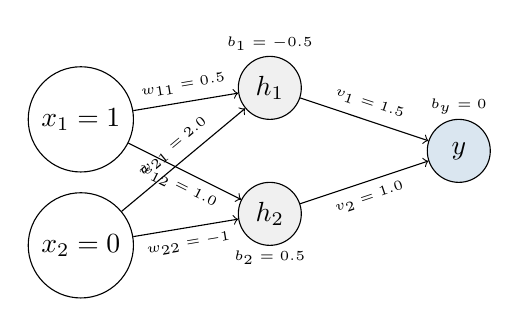
\begin{tikzpicture}[scale=0.8]
% Input nodes
\node[circle,draw,minimum size=0.8cm] (x1) at (0,2) {$x_1=1$};
\node[circle,draw,minimum size=0.8cm] (x2) at (0,0) {$x_2=0$};
% Hidden nodes
\node[circle,draw,fill=lightGray,minimum size=0.8cm] (h1) at (3,2.5) {$h_1$};
\node[circle,draw,fill=lightGray,minimum size=0.8cm] (h2) at (3,0.5) {$h_2$};
% Output node
\node[circle,draw,fill=checkpointBlue!20,minimum size=0.8cm] (y) at (6,1.5) {$y$};
% Connections with weights
\draw[->] (x1) -- node[above,sloped,font=\tiny] {$w_{11}=0.5$} (h1);
\draw[->] (x1) -- node[below,sloped,font=\tiny] {$w_{12}=1.0$} (h2);
\draw[->] (x2) -- node[above,sloped,font=\tiny] {$w_{21}=2.0$} (h1);
\draw[->] (x2) -- node[below,sloped,font=\tiny] {$w_{22}=-1$} (h2);
\draw[->] (h1) -- node[above,sloped,font=\tiny] {$v_1=1.5$} (y);
\draw[->] (h2) -- node[below,sloped,font=\tiny] {$v_2=1.0$} (y);
% Bias labels
\node[font=\tiny] at (3,3.2) {$b_1=-0.5$};
\node[font=\tiny] at (3,-0.2) {$b_2=0.5$};
\node[font=\tiny] at (6,2.2) {$b_y=0$};
\end{tikzpicture}
\end{center}

\textbf{Your Task:} Calculate the output!

\tryit{Fill in the blanks as we go:}
\begin{itemize}
\item $h_1 = ?$
\item $h_2 = ?$
\item $y = ?$
\end{itemize}

\column{0.42\textwidth}
\textbf{Step 1: Calculate Hidden Neurons}
\begin{align*}
h_1 &= \text{ReLU}(1 \cdot 0.5 + 0 \cdot 2.0 - 0.5) \\
    &= \text{ReLU}(0.5 + 0 - 0.5) \\
    &= \text{ReLU}(0) = \highlight{0}
\end{align*}

\begin{align*}
h_2 &= \text{ReLU}(1 \cdot 1.0 + 0 \cdot (-1) + 0.5) \\
    &= \text{ReLU}(1.0 + 0 + 0.5) \\
    &= \text{ReLU}(1.5) = \highlight{1.5}
\end{align*}

\textbf{Step 2: Calculate Output}
\begin{align*}
y &= 0 \cdot 1.5 + 1.5 \cdot 1.0 + 0 \\
  &= 0 + 1.5 + 0 = \highlight{1.5}
\end{align*}

\success{The network output is 1.5!}
\end{columns}
\vfill
\secondary{\footnotesize This is exactly what happens millions of times per second in deep learning}
\end{frame}

% NEW: XOR Solution Step-by-Step
\begin{frame}{Solving XOR: Step-by-Step with Hidden Layers}
\begin{center}
\includegraphics[width=0.95\textwidth]{../figures/xor_solution_steps.pdf}
\end{center}
\vfill
\secondary{\footnotesize Two simple linear boundaries combine to solve the impossible XOR problem}
\end{frame}

% NEW: Weight Update Visualization
\begin{frame}{Learning in Action: Weight Evolution}
\begin{center}
\includegraphics[width=0.9\textwidth]{../figures/weight_update_animation.pdf}
\end{center}
\vfill
\secondary{\footnotesize Watch as random weights organize into meaningful patterns through learning}
\end{frame}

% Backpropagation
\begin{frame}{1986: Backpropagation - Teaching Networks to Learn}
\begin{center}
\textbf{The Credit Assignment Problem: Who's to Blame?}
\end{center}
\vspace{5mm}
\begin{columns}
\column{0.48\textwidth}
\textbf{The Challenge:}
\begin{itemize}
\item Network makes error at output
\item Many neurons contributed
\item Which weights should change?
\item By how much?
\end{itemize}

\textbf{The Solution: Chain Rule}
\begin{itemize}
\item Calculate error at output
\item Propagate error backwards
\item Each layer gets its "share of blame"
\item Adjust weights proportionally
\end{itemize}

\column{0.48\textwidth}
\textbf{Mathematical Insight:}
$$\frac{\partial E}{\partial w_{ij}} = \frac{\partial E}{\partial out_j} \cdot \frac{\partial out_j}{\partial net_j} \cdot \frac{\partial net_j}{\partial w_{ij}}$$
\plainmath{How much should we change this weight? = How wrong were we? times How sensitive is the output? times How much did this weight contribute?}

\textbf{In Simple Terms:}
\begin{enumerate}
\item How wrong were we? (Error)
\item How sensitive is error to this weight?
\item Adjust weight in opposite direction
\item Repeat for all weights, back to front
\end{enumerate}
\end{columns}
\vfill
\secondary{\footnotesize This algorithm is still the foundation of all deep learning today}
\end{frame}

% NEW: NetTalk Success Story
\begin{frame}{1987: NetTalk - Networks Learn to Speak}
\begin{center}
\textbf{Sejnowski \& Rosenberg's Speaking Network}
\end{center}
\vspace{5mm}
\begin{columns}
\column{0.48\textwidth}
\textbf{The Challenge:}
\begin{itemize}
\item English pronunciation is irregular
\item "though" vs "through" vs "tough"
\item Rule-based systems failed
\item Can a network learn from examples?
\end{itemize}

\textbf{The Architecture:}
\begin{itemize}
\item Input: 7 letters (context window)
\item Hidden: 80 neurons
\item Output: 26 phonemes
\item 18,000 total weights
\end{itemize}

\column{0.48\textwidth}
\textbf{The Results:}
\begin{itemize}
\item Started: Random babbling
\item After 10 epochs: Consonants/vowels
\item After 30 epochs: Simple words
\item After 50 epochs: 95\% correct!
\end{itemize}

\textbf{Why It Mattered:}
\begin{itemize}
\item Proved backprop works on real problems
\item Learned complex, irregular mappings
\item No rules programmed!
\item Sounded like a child learning to read
\end{itemize}
\end{columns}
\vfill
\secondary{\footnotesize The network literally learned English pronunciation overnight}
\end{frame}

% NEW: Universal Approximation Theorem
\begin{frame}{1989: Universal Approximation - The Mathematical Foundation}
\begin{center}
\textbf{Cybenko's Theorem: Networks Can Learn ANY Function}
\end{center}
\vspace{5mm}
\begin{columns}
\column{0.48\textwidth}
\textbf{The Theorem:}
"A feedforward network with:
\begin{itemize}
\item One hidden layer
\item Finite neurons
\item Sigmoid activation
\end{itemize}
can approximate ANY continuous function to arbitrary accuracy"

\textbf{What This Means:}
\begin{itemize}
\item Neural networks are universal
\item Can solve any pattern recognition
\item Just need enough neurons
\item Mathematics guarantees it!
\end{itemize}

\column{0.48\textwidth}
\textbf{The Catch:}
\begin{itemize}
\item Doesn't say HOW MANY neurons
\item Doesn't say HOW to find weights
\item Might need exponentially many
\item Training might take forever
\end{itemize}

\textbf{Historical Impact:}
\begin{itemize}
\item Ended theoretical doubts
\item Justified deep learning research
\item Shifted focus to practical training
\item "We know it's possible, now make it work"
\end{itemize}
\end{columns}
\vfill
\secondary{\footnotesize This theorem convinced skeptics that neural networks were worth pursuing}
\end{frame}

% NEW: The Vanishing Gradient Problem
\begin{frame}{The Vanishing Gradient Problem: Why Deep Was Hard}
\begin{center}
\includegraphics[width=0.95\textwidth]{../figures/vanishing_gradient_flow.pdf}
\end{center}
\vfill
\secondary{\footnotesize Gradients shrink exponentially through layers---this blocked deep learning until ReLU (2011)}
\end{frame}

% NEW: Try It Yourself - Backprop Intuition
\begin{frame}{Try It Yourself: Understanding Backpropagation}
\begin{center}
\textbf{\checkpoint{Let's Work Through a Tiny Example}}
\end{center}
\vspace{5mm}
\begin{columns}
\column{0.48\textwidth}
\textbf{Simple 2-Layer Network:}
\begin{itemize}
\item Input: 1
\item Weight 1: 2 (makes it 2)
\item Weight 2: 3 (makes it 6)
\item Target output: 10
\item Actual output: 6
\item Error: 4
\end{itemize}

\tryit{If we're off by 4, and weight 2 multiplies by 3, how much should we adjust weight 2? What about weight 1?}

\column{0.48\textwidth}
\textbf{The Intuition:}
\begin{enumerate}
\item Error at output: -4 (too small)
\item Weight 2's fault: It multiplied by 3
\item Adjust weight 2: Add ~1.3
\item Weight 1's fault: Fed into weight 2
\item Adjust weight 1: Smaller change
\end{enumerate}

\textbf{Key Insight:}
\begin{itemize}
\item Closer to output = bigger updates
\item Further back = smaller updates
\item This is the "chain rule" in action!
\end{itemize}
\end{columns}
\vfill
\secondary{\footnotesize This simple idea scales to billions of parameters}
\end{frame}

% Activation Functions
\begin{frame}{Why Linear Doesn't Work: Activation Functions}
\begin{center}
\textbf{The Need for Non-Linearity}
\end{center}
\vspace{5mm}
\begin{columns}
\column{0.48\textwidth}
\textbf{Problem with Linear:}
\begin{itemize}
\item Stack of linear layers = still linear!
\item $f(g(x)) = (wx + b_1)w' + b_2 = w'wx + ...$
\item Can't learn complex patterns
\end{itemize}

\textbf{Solution: Activation Functions}
\begin{itemize}
\item Add non-linearity after each layer
\item Allows learning complex boundaries
\item Different functions for different needs
\end{itemize}

\column{0.48\textwidth}
\textbf{Common Activation Functions:}
\begin{itemize}
\item \textbf{Sigmoid:} $\sigma(x) = \frac{1}{1 + e^{-x}}$
   \begin{itemize}
   \item Smooth, outputs 0-1
   \item Good for probabilities
   \end{itemize}
   \plainmath{Squashes any input to range 0-1. Large positive becomes 1, large negative becomes 0}
\item \textbf{ReLU:} $f(x) = \max(0, x)$
   \begin{itemize}
   \item Simple, fast
   \item Solves vanishing gradient
   \end{itemize}
\item \textbf{Tanh:} $\tanh(x) = \frac{e^x - e^{-x}}{e^x + e^{-x}}$
   \begin{itemize}
   \item Outputs -1 to 1
   \item Zero-centered
   \end{itemize}
\end{itemize}
\end{columns}
\vfill
\secondary{\footnotesize ReLU's simplicity revolutionized deep learning in 2011}
\end{frame}

% Simple 2D Example
\begin{frame}{Visualizing Learning: 2D Classification}
\begin{center}
\textbf{Teaching a Network to Separate Red from Blue Points}
\end{center}
\vspace{5mm}
\begin{columns}
\column{0.48\textwidth}
\textbf{The Setup:}
\begin{itemize}
\item Input: (x, y) coordinates
\item Output: Red or Blue class
\item Network: 2 $\rightarrow$ 4 $\rightarrow$ 2 neurons
\end{itemize}

\textbf{Training Process:}
\begin{enumerate}
\item Epoch 1: Random boundary
\item Epoch 10: Rough separation
\item Epoch 50: Good boundary
\item Epoch 100: Perfect fit
\end{enumerate}

\column{0.48\textwidth}
\begin{center}
\includegraphics[width=\textwidth]{../figures/2d_classification_evolution.pdf}
\end{center}
\textbf{What Each Layer Learns:}
\begin{itemize}
\item Layer 1: Simple boundaries
\item Hidden: Combine boundaries
\item Output: Final decision
\end{itemize}
\end{columns}
\vfill
\secondary{\footnotesize This same principle scales to millions of parameters}
\end{frame}

% Act III: The Breakthrough
\begin{frame}{Act III: The Breakthrough Years}
\begin{center}
{\Large \textbf{1998-2012: From Digits to ImageNet}}
\end{center}
\vspace{5mm}
\begin{columns}
\column{0.48\textwidth}
\textbf{1998 - LeNet: First Success}
\begin{itemize}
\item Yann LeCun's CNN for digits
\item 32$\times$32 pixels $\rightarrow$ 10 classes
\item 60,000 parameters
\item Banks adopt for check reading
\end{itemize}

\textbf{Key Innovation: Convolutions}
\begin{itemize}
\item Share weights across image
\item Detect features anywhere
\item Build complexity layer by layer
\end{itemize}

\column{0.48\textwidth}
\textbf{2012 - AlexNet: The Revolution}
\begin{itemize}
\item 1000 ImageNet classes
\item 60 million parameters
\item GPUs enable training
\item Error rate: 26\% $\rightarrow$ 16\%
\end{itemize}

\textbf{What Changed:}
\begin{itemize}
\item Big Data (millions of images)
\item GPU computing (100x faster)
\item ReLU activation
\item Dropout regularization
\end{itemize}
\end{columns}
\vfill
\secondary{\footnotesize This victory ended the second AI winter permanently}
\end{frame}

% Understanding Convolutions
\begin{frame}{The Convolution Innovation: See Like Humans Do}
\begin{center}
\textbf{How We Actually Recognize Objects}
\end{center}
\vspace{5mm}
\begin{columns}
\column{0.48\textwidth}
\textbf{Human Vision Process:}
\begin{enumerate}
\item Detect edges
\item Find shapes
\item Identify parts
\item Recognize object
\end{enumerate}

\textbf{CNN Mimics This:}
\begin{itemize}
\item Layer 1: Edge detectors
\item Layer 2: Corner/curve detectors
\item Layer 3: Part detectors
\item Layer 4: Object detectors
\end{itemize}

\column{0.48\textwidth}
\begin{center}
\includegraphics[width=\textwidth]{../figures/cnn_feature_hierarchy.pdf}
\end{center}
\textbf{Key Insight:}
\begin{itemize}
\item A "wheel detector" works anywhere in image
\item Share the same detector across positions
\item Reduces parameters dramatically
\item Makes network translation-invariant
\end{itemize}
\end{columns}
\vfill
\secondary{\footnotesize This is why CNNs dominate computer vision}
\end{frame}

% The Mathematics of Learning
\begin{frame}{The Mathematics of Learning: Gradient Descent}
\begin{center}
\textbf{Finding the Best Weights: Like Hiking Down a Mountain}
\end{center}
\vspace{5mm}
\begin{columns}
\column{0.48\textwidth}
\textbf{The Optimization Problem:}
\begin{itemize}
\item Millions of weights to adjust
\item Each affects the error
\item Need to find best combination
\end{itemize}

\textbf{Gradient Descent:}
\begin{enumerate}
\item Calculate error (loss)
\item Find slope (gradient) for each weight
\item Step downhill: $w = w - \alpha \cdot \nabla L$
   \plainmath{New weight = old weight - (step size times slope)}
\item Repeat until bottom
\end{enumerate}

\column{0.48\textwidth}
\begin{center}
\includegraphics[width=\textwidth]{../figures/gradient_descent.pdf}
\end{center}
\textbf{Learning Rate ($\alpha$):}
\begin{itemize}
\item Too small: takes forever
\item Too large: overshoot minimum
\item Just right: smooth convergence
\end{itemize}
\end{columns}
\vfill
\secondary{\footnotesize Modern optimizers like Adam adapt the learning rate automatically}
\end{frame}

% Types of Learning
\begin{frame}{Types of Learning: Different Problems, Different Approaches}
\begin{columns}
\column{0.48\textwidth}
\textbf{Supervised Learning:}
\begin{itemize}
\item Have input-output pairs
\item Learn mapping function
\item Examples: Classification, Regression
\end{itemize}

\textbf{Unsupervised Learning:}
\begin{itemize}
\item Only have inputs
\item Find patterns/structure
\item Examples: Clustering, Compression
\end{itemize}

\column{0.48\textwidth}
\textbf{Reinforcement Learning:}
\begin{itemize}
\item Learn through trial/error
\item Maximize reward signal
\item Examples: Games, Robotics
\end{itemize}

\textbf{Self-Supervised (Modern):}
\begin{itemize}
\item Create labels from data itself
\item Predict next word, masked words
\item Examples: GPT, BERT
\end{itemize}
\end{columns}
\vfill
\secondary{\footnotesize Self-supervised learning powers all modern language models}
\end{frame}

% NEW: Understanding Checkpoint - Types of Learning
\begin{frame}{Check Your Understanding: Learning Types}
\begin{center}
\textbf{\checkpoint{Can You Match These Examples?}}
\end{center}
\vspace{5mm}
\tryit{Match each scenario to a learning type: Supervised, Unsupervised, Reinforcement, Self-Supervised}
\vspace{5mm}
\begin{columns}
\column{0.48\textwidth}
\textbf{Scenarios:}
\begin{enumerate}
\item Teaching a robot to walk by giving rewards for standing
\item Showing 1000 cat photos labeled "cat"
\item Giving GPT text with words masked out
\item Finding groups in customer data
\end{enumerate}

\column{0.48\textwidth}
\textbf{Answers:}
\begin{enumerate}
\item Reinforcement (trial and error)
\item Supervised (labeled examples)
\item Self-supervised (creates own labels)
\item Unsupervised (finds patterns)
\end{enumerate}

\confusion{Self-supervised IS supervised learning - we just create the labels automatically from the data itself!}
\end{columns}
\vfill
\secondary{\footnotesize Understanding these differences helps you choose the right approach}
\end{frame}

% Overfitting Problem
\begin{frame}{The Overfitting Problem: When Learning Goes Too Far}
\begin{center}
\textbf{Memorization vs. Understanding}
\end{center}
\vspace{5mm}
\begin{columns}
\column{0.48\textwidth}
\textbf{The Problem:}
\begin{itemize}
\item Network memorizes training data
\item Fails on new, unseen data
\item Like student memorizing answers
\end{itemize}

\textbf{Signs of Overfitting:}
\begin{itemize}
\item Training accuracy: 99\%
\item Test accuracy: 60\%
\item Complex decision boundaries
\item High variance
\end{itemize}

\column{0.48\textwidth}
\begin{center}
\includegraphics[width=\textwidth]{../figures/overfitting_visualization.pdf}
\end{center}
\textbf{Solutions:}
\begin{itemize}
\item \textbf{More data:} Can't memorize everything
\item \textbf{Dropout:} Randomly disable neurons
\item \textbf{Regularization:} Penalize complexity
\item \textbf{Early stopping:} Stop before overfitting
\end{itemize}
\end{columns}
\vfill
\secondary{\footnotesize "With four parameters I can fit an elephant, with five I can make him wiggle his trunk" - von Neumann}
\end{frame}

% NEW: Feature Hierarchy Progression
\begin{frame}{How Deep Networks See: Building Features Layer by Layer}
\begin{center}
\textbf{From Pixels to Concepts: The Hierarchy of Understanding}
\end{center}
\vspace{5mm}
\begin{columns}
\column{0.55\textwidth}
\includegraphics[width=\textwidth]{../figures/feature_hierarchy_progression.pdf}

\textbf{What Each Layer Learns:}
\begin{itemize}
\item \textbf{Layer 1:} Edges, colors, gradients
\item \textbf{Layer 2:} Corners, textures, curves
\item \textbf{Layer 3:} Parts (eyes, wheels, patterns)
\item \textbf{Layer 4:} Objects (faces, cars, scenes)
\item \textbf{Layer 5:} Concepts (identity, style, context)
\end{itemize}

\column{0.42\textwidth}
\textbf{Why Hierarchy Matters:}
\begin{itemize}
\item Reusable features
\item Efficient representation
\item Transfer learning works
\item Mimics visual cortex
\end{itemize}

\textbf{Discovered Automatically:}
\begin{itemize}
\item No manual feature engineering
\item Emerges from data
\item Different tasks, same hierarchy
\item Universal pattern
\end{itemize}
\end{columns}
\vfill
\secondary{\footnotesize Each layer combines features from the previous layer into more abstract concepts}
\end{frame}

% NEW: Training Dynamics Dashboard
\begin{frame}{Training Dynamics: Watching Networks Learn}
\begin{center}
\textbf{Real-Time Monitoring: The Training Dashboard}
\end{center}
\vspace{3mm}
\begin{columns}
\column{0.55\textwidth}
\includegraphics[width=\textwidth]{../figures/training_dynamics_dashboard.pdf}

\textbf{Key Metrics to Track:}
\begin{itemize}
\item \textbf{Loss Curves:} Training vs validation
\item \textbf{Accuracy:} How often we're right
\item \textbf{Learning Rate:} Speed of updates
\item \textbf{Gradient Norm:} Update magnitude
\end{itemize}

\column{0.42\textwidth}
\textbf{Warning Signs:}
\begin{itemize}
\item Gap = Overfitting
\item Flat = Learning stopped
\item Spikes = Instability
\item NaN = Numerical issues
\end{itemize}

\textbf{Healthy Training:}
\begin{itemize}
\item Smooth decrease
\item Val follows train
\item Gradients stable
\item LR decays properly
\end{itemize}

\textbf{When to Stop:}
\begin{itemize}
\item Validation plateaus
\item Gap increasing
\item Diminishing returns
\end{itemize}
\end{columns}
\vfill
\secondary{\footnotesize Modern training requires constant monitoring - it's more art than science}
\end{frame}

% Act IV: The Revolution
\begin{frame}{Act IV: The Deep Learning Revolution}
\begin{center}
{\Large \textbf{2014-Present: Networks That Changed the World}}
\end{center}
\vspace{5mm}
\begin{columns}
\column{0.48\textwidth}
\textbf{The Depth Revolution:}
\begin{itemize}
\item 2014 - VGGNet: 19 layers
\item 2015 - ResNet: 152 layers
\item 2017 - Transformers: Attention
\item 2020 - GPT-3: 175B parameters
\end{itemize}

\textbf{Why Depth Matters:}
\begin{itemize}
\item Each layer = abstraction level
\item Deep = complex reasoning
\item Hierarchical feature learning
\end{itemize}

\column{0.48\textwidth}
\textbf{Real-World Impact:}
\begin{itemize}
\item \textbf{Vision:} Self-driving cars
\item \textbf{Language:} Google Translate
\item \textbf{Speech:} Siri, Alexa
\item \textbf{Medicine:} Disease diagnosis
\item \textbf{Science:} Protein folding
\end{itemize}

\textbf{The Scale:}
\begin{itemize}
\item Billions of parameters
\item Trained on internet-scale data
\item Months of GPU time
\item Emergent abilities appear
\end{itemize}
\end{columns}
\vfill
\secondary{\footnotesize We went from recognizing digits to passing the bar exam in 25 years}
\end{frame}

% ResNet Innovation
\begin{frame}{2015: ResNet - The Skip Connection Revolution}
\begin{center}
\textbf{Problem: Networks Couldn't Get Deeper}
\end{center}
\vspace{5mm}
\begin{columns}
\column{0.48\textwidth}
\textbf{The Vanishing Gradient:}
\begin{itemize}
\item Gradients multiply through layers
\item Become exponentially small
\item Deep layers stop learning
\item 20 layers was the limit
\end{itemize}

\textbf{The Breakthrough: Skip Connections}
\begin{itemize}
\item Add input directly to output
\item $F(x) + x$ instead of just $F(x)$
\item Gradients flow directly backward
\item Can train 1000+ layers!
\end{itemize}

\column{0.48\textwidth}
\begin{center}
\includegraphics[width=\textwidth]{../figures/resnet_skip_connection.pdf}
\end{center}
\textbf{Why It Works:}
\begin{itemize}
\item Learn residual (difference) only
\item Identity mapping is easy default
\item Gradients have direct path
\item Each layer refines previous result
\end{itemize}
\end{columns}
\vfill
\secondary{\footnotesize This simple trick enabled the deep learning revolution}
\end{frame}

% Batch Normalization
\begin{frame}{Batch Normalization: Keeping Networks Stable}
\begin{center}
\textbf{The Internal Covariate Shift Problem}
\end{center}
\vspace{5mm}
\begin{columns}
\column{0.48\textwidth}
\textbf{The Issue:}
\begin{itemize}
\item Each layer's input distribution changes
\item As previous layers update
\item Makes learning unstable
\item Requires tiny learning rates
\end{itemize}

\textbf{The Solution:}
\begin{itemize}
\item Normalize inputs to each layer
\item Mean = 0, Variance = 1
\item Learn scale and shift parameters
\item Apply during training and testing
\end{itemize}

\column{0.48\textwidth}
\textbf{BatchNorm Algorithm:}
\begin{align*}
\mu_B &= \frac{1}{m} \sum_{i=1}^{m} x_i \\
\sigma_B^2 &= \frac{1}{m} \sum_{i=1}^{m} (x_i - \mu_B)^2 \\
\hat{x}_i &= \frac{x_i - \mu_B}{\sqrt{\sigma_B^2 + \epsilon}} \\
y_i &= \gamma \hat{x}_i + \beta
\end{align*}
\plainmath{1) Find average, 2) Find spread, 3) Normalize to standard range, 4) Scale and shift as needed}

\textbf{Benefits:}
\begin{itemize}
\item 10x faster training
\item Higher learning rates OK
\item Less sensitive to initialization
\item Acts as regularization
\end{itemize}
\end{columns}
\vfill
\secondary{\footnotesize Now standard in every deep network}
\end{frame}

% NEW: The Lottery Ticket Hypothesis
\begin{frame}{2019: The Lottery Ticket Hypothesis}
\begin{center}
\textbf{Most Network Weights Don't Matter!}
\end{center}
\vspace{5mm}
\begin{columns}
\column{0.48\textwidth}
\textbf{The Discovery:}
\begin{itemize}
\item Networks contain "winning tickets"
\item Subnetworks that train well alone
\item 90-95\% of weights can be removed
\item Performance stays the same!
\end{itemize}

\textbf{The Hypothesis:}
"Dense networks succeed because they contain sparse subnetworks that are capable of training effectively"

\column{0.48\textwidth}
\textbf{Implications:}
\begin{itemize}
\item We massively overparameterize
\item Training finds the needle in haystack
\item Future: Train small from start?
\item Mobile deployment possible
\end{itemize}

\textbf{Why It Matters:}
\begin{itemize}
\item Explains why big networks train better
\item Pruning after training works
\item Efficiency revolution starting
\item Changes how we think about learning
\end{itemize}
\end{columns}
\vfill
\secondary{\footnotesize A 1 billion parameter model might only need 50 million}
\end{frame}

% NEW: Inductive Biases
\begin{frame}{Inductive Biases: Building in Assumptions}
\begin{center}
\textbf{The Right Architecture for the Right Problem}
\end{center}
\vspace{5mm}
\begin{columns}
\column{0.48\textwidth}
\textbf{What Are Inductive Biases?}
\begin{itemize}
\item Assumptions built into architecture
\item Guide learning toward solutions
\item Trade flexibility for efficiency
\item "Priors" about the problem
\end{itemize}

\textbf{Examples:}
\begin{itemize}
\item \textbf{CNN:} Spatial locality matters
\item \textbf{RNN:} Order/time matters
\item \textbf{GNN:} Graph structure matters
\item \textbf{Transformer:} All positions can interact
\end{itemize}

\column{0.48\textwidth}
\textbf{Why They Matter:}
\begin{itemize}
\item Reduce search space
\item Faster convergence
\item Better generalization
\item Less data needed
\end{itemize}

\textbf{The Tradeoff:}
\begin{itemize}
\item Right bias = 10x better
\item Wrong bias = 10x worse
\item General architectures = safe but slow
\item Specialized = fast but limited
\end{itemize}
\end{columns}
\vfill
\secondary{\footnotesize Choosing the right inductive bias is still an art}
\end{frame}

% NEW: Emergent Abilities
\begin{frame}{Emergent Abilities: When Scale Creates Intelligence}
\begin{center}
\textbf{Capabilities That Appear Suddenly with Scale}
\end{center}
\vspace{5mm}
\begin{columns}
\column{0.48\textwidth}
\textbf{The Phenomenon:}
\begin{itemize}
\item Small models: Can't do task at all
\item Medium models: Still can't
\item Large models: Suddenly can!
\item No gradual improvement
\end{itemize}

\textbf{Examples:}
\begin{itemize}
\item 3-digit arithmetic (>10B params)
\item Chain-of-thought reasoning (>50B)
\item Code generation (>20B)
\item Multilingual translation (>100B)
\end{itemize}

\column{0.48\textwidth}
\textbf{Why It Happens:}
\begin{itemize}
\item Complex patterns need capacity
\item Phase transitions in learning
\item Composition of simpler abilities
\item "Grokking" - sudden understanding
\end{itemize}

\textbf{Implications:}
\begin{itemize}
\item We can't predict what's next
\item Scaling might unlock AGI
\item Or hit fundamental limits
\item Active area of research
\end{itemize}
\end{columns}
\vfill
\secondary{\footnotesize GPT-3 showed abilities nobody expected or programmed}
\end{frame}

% NEW: Depth vs Width Comparison
\begin{frame}{Architecture Choices: Deep vs Wide Networks}
\begin{center}
\textbf{The Fundamental Tradeoff in Neural Architecture}
\end{center}
\vspace{5mm}
\begin{columns}
\column{0.55\textwidth}
\includegraphics[width=\textwidth]{../figures/depth_width_comparison.pdf}

\textbf{Deep Networks (Many Layers):}
\begin{itemize}
\item Complex hierarchical features
\item Exponential expressiveness growth
\item Harder to train (vanishing gradients)
\item Better for vision, NLP
\end{itemize}

\textbf{Wide Networks (Many Neurons):}
\begin{itemize}
\item More parallel processing
\item Easier optimization landscape
\item Linear expressiveness growth
\item Better for tabular data
\end{itemize}

\column{0.42\textwidth}
\textbf{The Sweet Spot:}
\begin{itemize}
\item Vision: Deep (100+ layers)
\item Language: Very deep (24-96 layers)
\item Tabular: Wide and shallow (2-4 layers)
\item Time series: Moderate (5-10 layers)
\end{itemize}

\textbf{Modern Insights:}
\begin{itemize}
\item Depth beats width for same parameters
\item Skip connections enable extreme depth
\item Width helps with memorization
\item Depth helps with generalization
\end{itemize}

\textbf{Scaling Laws:}
\begin{itemize}
\item Performance $\propto$ depth$^{0.8}$
\item Performance $\propto$ width$^{0.5}$
\end{itemize}
\end{columns}
\vfill
\secondary{\footnotesize The depth revolution (2012-2016) showed that deep beats wide for most problems}
\end{frame}

% NEW: Data Scaling Laws
\begin{frame}{Scaling Laws: How Performance Grows with Data}
\begin{center}
\textbf{The Predictable Relationship Between Data, Model Size, and Performance}
\end{center}
\vspace{5mm}
\begin{columns}
\column{0.55\textwidth}
\includegraphics[width=\textwidth]{../figures/data_scaling_laws.pdf}

\textbf{The Chinchilla Law (2022):}
\begin{itemize}
\item Optimal ratio: 20 tokens per parameter
\item 10B model needs 200B tokens
\item Most models are undertrained
\item Data quality matters more than quantity
\end{itemize}

\textbf{Power Law Scaling:}
$$\text{Loss} = A \cdot N^{-\alpha} + B \cdot D^{-\beta} + C$$
\begin{itemize}
\item $N$ = model parameters
\item $D$ = dataset size
\item $\alpha \approx 0.07$, $\beta \approx 0.10$
\end{itemize}

\column{0.42\textwidth}
\textbf{Practical Implications:}
\begin{itemize}
\item 10x data $\rightarrow$ 2x performance
\item 10x parameters $\rightarrow$ 1.7x performance
\item 10x compute $\rightarrow$ 3x performance
\item Diminishing returns always
\end{itemize}

\textbf{Data Efficiency Tricks:}
\begin{itemize}
\item Data augmentation
\item Synthetic data generation
\item Active learning
\item Curriculum learning
\item Multi-task training
\end{itemize}

\whymatters{These laws predict costs before training}

\textbf{Current Limits:}
\begin{itemize}
\item Internet has ~10T tokens
\item Already using most of it
\item Quality > Quantity now
\end{itemize}
\end{columns}
\vfill
\secondary{\footnotesize These laws let us predict performance before training - saving millions in compute}
\end{frame}

% NEW: Optimizer Comparison
\begin{frame}{Optimization Algorithms: How Networks Learn}
\begin{center}
\textbf{The Evolution of Gradient Descent}
\end{center}
\vspace{5mm}
\begin{columns}
\column{0.55\textwidth}
\includegraphics[width=\textwidth]{../figures/optimizer_comparison.pdf}

\textbf{SGD (1951):}
\begin{itemize}
\item Basic gradient descent
\item Learning rate: Fixed
\item Slow but reliable
\item Still used for fine-tuning
\end{itemize}

\textbf{Momentum (1964):}
\begin{itemize}
\item Remember past gradients
\item Accelerate in consistent directions
\item Escape shallow local minima
\item $v_t = \beta v_{t-1} + (1-\beta) g_t$
\end{itemize}

\column{0.42\textwidth}
\textbf{Adam (2014):}
\begin{itemize}
\item Adaptive learning rates per parameter
\item Combines momentum + RMSprop
\item De facto standard
\item Works out-of-the-box
\end{itemize}

\textbf{Modern Variants:}
\begin{itemize}
\item \textbf{AdamW:} Decoupled weight decay
\item \textbf{RAdam:} Rectified Adam
\item \textbf{LAMB:} Large batch training
\item \textbf{Sophia:} 2nd-order approximation
\end{itemize}

\textbf{Choosing an Optimizer:}
\begin{itemize}
\item Start with Adam (lr=3e-4)
\item Large batch: LAMB
\item Fine-tuning: SGD with momentum
\item Transformers: AdamW
\end{itemize}
\end{columns}
\vfill
\secondary{\footnotesize Adam works 90\% of the time - but that last 10\% matters for SOTA results}
\end{frame}

% NEW: Architecture Decision Tree
\begin{frame}{Quick Guide: Choosing Your Architecture}
\begin{center}
\textbf{\checkpoint{Which Network Should You Use?}}
\end{center}
\vspace{5mm}
\begin{columns}
\column{0.55\textwidth}
\includegraphics[width=\textwidth]{../figures/architecture_decision_tree.pdf}

\tryit{You have 10,000 customer reviews to classify as positive/negative. Which architecture? Why?}

\column{0.42\textwidth}
\textbf{Decision Questions:}
\begin{enumerate}
\item Is your data sequential?
\item Does position matter?
\item Is it images/spatial?
\item Fixed or variable size?
\end{enumerate}

\textbf{Quick Rules:}
\begin{itemize}
\item Images $\rightarrow$ CNN
\item Text $\rightarrow$ Transformer/RNN
\item Tabular $\rightarrow$ Feedforward
\item Audio $\rightarrow$ CNN or RNN
\item Video $\rightarrow$ CNN + RNN
\end{itemize}

\confusion{Transformers now dominate most tasks, but specialized architectures still win for specific problems!}
\end{columns}
\vfill
\secondary{\footnotesize Answer: Transformer or RNN - text is sequential and context matters}
\end{frame}

% Different Architectures
\begin{frame}{Neural Network Architectures: Right Tool for Right Job}
\begin{columns}
\column{0.48\textwidth}
\textbf{Feedforward Networks:}
\begin{itemize}
\item Information flows forward only
\item Fixed-size input and output
\item Good for: Classification, regression
\end{itemize}

\textbf{Convolutional (CNN):}
\begin{itemize}
\item Spatial feature detection
\item Translation invariance
\item Good for: Images, video
\end{itemize}

\column{0.48\textwidth}
\textbf{Recurrent (RNN):}
\begin{itemize}
\item Process sequences
\item Maintain memory/state
\item Good for: Text, time-series
\end{itemize}

\textbf{Transformer:}
\begin{itemize}
\item Attention mechanism
\item Parallel processing
\item Good for: Language, everything else
\end{itemize}
\end{columns}
\vfill
\secondary{\footnotesize Each architecture encodes different assumptions about the data}
\end{frame}

% Modern Training Techniques
\begin{frame}{Modern Training: Standing on Shoulders of Giants}
\begin{columns}
\column{0.48\textwidth}
\textbf{Transfer Learning:}
\begin{itemize}
\item Start with pre-trained network
\item Fine-tune on your task
\item 100x less data needed
\item Days $\rightarrow$ Hours training
\end{itemize}

\textbf{Data Augmentation:}
\begin{itemize}
\item Create variations of training data
\item Rotations, crops, color shifts
\item Prevents overfitting
\item Free performance boost
\end{itemize}

\column{0.48\textwidth}
\textbf{Advanced Optimizers:}
\begin{itemize}
\item \textbf{SGD:} Basic gradient descent
\item \textbf{Momentum:} Remember past gradients
\item \textbf{Adam:} Adaptive learning rates
\item \textbf{AdamW:} With weight decay
\end{itemize}

\textbf{Mixed Precision:}
\begin{itemize}
\item Use 16-bit floats where possible
\item Keep 32-bit for critical ops
\item 2-3x speedup
\item Same accuracy
\end{itemize}
\end{columns}
\vfill
\secondary{\footnotesize These techniques make deep learning practical for everyone}
\end{frame}

% NEW: Common Mental Models That Are WRONG
\begin{frame}{Common Mental Models That Are WRONG}
\begin{center}
\textbf{\warning{Misconceptions That Will Confuse You}}
\end{center}
\vspace{5mm}
\begin{columns}
\column{0.48\textwidth}
\textbf{WRONG: "Neurons are like brain neurons"}
\begin{itemize}
\item \warning{Brain neurons:} Complex, chemical, adaptive
\item \success{Artificial neurons:} Simple math functions
\item Just multiply and add!
\item No biology involved
\end{itemize}

\vspace{3mm}
\textbf{WRONG: "Networks understand concepts"}
\begin{itemize}
\item \warning{What you think:} "It knows what a cat is"
\item \success{Reality:} It found statistical patterns
\item No understanding, just correlation
\item Can be fooled by tiny changes
\end{itemize}

\column{0.48\textwidth}
\textbf{WRONG: "More layers = always better"}
\begin{itemize}
\item \warning{Too deep:} Vanishing gradients
\item \warning{Too deep:} Overfitting
\item \success{Right depth:} Depends on problem complexity
\item Simple problems need shallow networks
\end{itemize}

\vspace{3mm}
\textbf{WRONG: "It learns like humans"}
\begin{itemize}
\item \warning{Humans:} Learn from few examples
\item \warning{Humans:} Transfer knowledge easily
\item \success{Networks:} Need thousands of examples
\item \success{Networks:} Struggle with new situations
\end{itemize}
\end{columns}

\vspace{5mm}
\begin{center}
\colorbox{warningOrange!20}{\parbox{0.8\textwidth}{
\centering
\textbf{Remember:} Neural networks are just fancy pattern matchers.\\
They don't think, understand, or reason - they find correlations in data.
}}
\end{center}
\vfill
\secondary{\footnotesize Understanding these limits helps you use neural networks effectively}
\end{frame}

% Why Now?
\begin{frame}{Why Deep Learning Exploded Now: The Perfect Storm}
\begin{columns}
\column{0.48\textwidth}
\textbf{1. Data Explosion:}
\begin{itemize}
\item Internet = infinite training data
\item ImageNet: 14M labeled images
\item Common Crawl: 300TB of text
\item YouTube: 500 hours/minute
\end{itemize}

\textbf{2. Hardware Revolution:}
\begin{itemize}
\item GPUs: 100x faster than CPUs
\item TPUs: Built for neural nets
\item Cloud computing: Rent supercomputers
\item Mobile chips with NPUs
\end{itemize}

\column{0.48\textwidth}
\textbf{3. Algorithm Breakthroughs:}
\begin{itemize}
\item ReLU activation (2011)
\item Batch normalization (2015)
\item Skip connections (2015)
\item Attention mechanism (2017)
\end{itemize}

\textbf{4. Open Source Culture:}
\begin{itemize}
\item TensorFlow, PyTorch free
\item Pre-trained models shared
\item Papers with code
\item Collaborative research
\end{itemize}
\end{columns}
\vfill
\secondary{\footnotesize The same ideas from 1980s finally had the resources to work}
\end{frame}

% Understanding Scale
\begin{frame}{Understanding Scale: From Perceptron to GPT-4}
\begin{center}
\textbf{The Exponential Growth of Neural Networks}
\end{center}
\vspace{5mm}
\begin{columns}
\column{0.48\textwidth}
\textbf{Parameter Growth:}
\begin{itemize}
\item 1957 Perceptron: 20 weights
\item 1987 NetTalk: 18,000
\item 1998 LeNet: 60,000
\item 2012 AlexNet: 60 million
\item 2018 BERT: 340 million
\item 2020 GPT-3: 175 billion
\item 2023 GPT-4: ~1.8 trillion
\end{itemize}

\column{0.48\textwidth}
\begin{center}
\includegraphics[width=\textwidth]{../figures/scale_growth_chart.pdf}
\end{center}
\textbf{What Scale Brings:}
\begin{itemize}
\item Emergent abilities
\item Zero-shot learning
\item Multi-task capability
\item Common sense reasoning
\end{itemize}
\end{columns}
\vfill
\secondary{\footnotesize Each 10x increase unlocks new capabilities}
\end{frame}

% Practical Implementation
\begin{frame}[fragile]{From Theory to Practice: Your First Network}
\begin{center}
\textbf{Building a Digit Classifier in 10 Lines}
\end{center}
\vspace{5mm}
\begin{columns}
\column{0.58\textwidth}
\textbf{PyTorch Implementation:}
\begin{lstlisting}[language=Python,basicstyle=\tiny]
import torch
import torch.nn as nn

class SimpleNet(nn.Module):
    def __init__(self):
        super().__init__()
        self.fc1 = nn.Linear(784, 128)
        self.fc2 = nn.Linear(128, 10)

    def forward(self, x):
        x = torch.relu(self.fc1(x))
        return self.fc2(x)

# Train
model = SimpleNet()
optimizer = torch.optim.Adam(model.parameters())
criterion = nn.CrossEntropyLoss()
\end{lstlisting}

\column{0.38\textwidth}
\textbf{What This Does:}
\begin{itemize}
\item Input: 28$\times$28 pixel image
\item Hidden: 128 neurons
\item Output: 10 digit classes
\item Activation: ReLU
\item Training: Adam optimizer
\end{itemize}

\textbf{Training Loop:}
\begin{itemize}
\item Forward pass
\item Calculate loss
\item Backward pass
\item Update weights
\item Repeat
\end{itemize}
\end{columns}
\vfill
\secondary{\footnotesize This simple network achieves 97\% accuracy on MNIST}
\end{frame}

% NEW: Advanced Debugging Techniques
\begin{frame}{Debugging Neural Networks: Detective Work}
\begin{center}
\textbf{When Things Go Wrong (They Always Do)}
\end{center}
\vspace{5mm}
\begin{columns}
\column{0.48\textwidth}
\textbf{Gradient Issues:}
\begin{itemize}
\item \textbf{Exploding:} Gradients $\rightarrow$ infinity
   \begin{itemize}
   \item Solution: Gradient clipping
   \end{itemize}
\item \textbf{Vanishing:} Gradients $\rightarrow$ 0
   \begin{itemize}
   \item Solution: Better initialization, ReLU
   \end{itemize}
\item \textbf{Dead ReLU:} Neurons never activate
   \begin{itemize}
   \item Solution: LeakyReLU, smaller learning rate
   \end{itemize}
\end{itemize}

\textbf{Debugging Tools:}
\begin{itemize}
\item TensorBoard: Visualize training
\item Gradient histograms
\item Activation distributions
\item Weight evolution plots
\end{itemize}

\column{0.48\textwidth}
\textbf{Common Failure Modes:}
\begin{itemize}
\item Loss not decreasing: Learning rate
\item Loss NaN: Numerical instability
\item Oscillating loss: LR too high
\item Plateau: Local minimum or LR too small
\end{itemize}

\textbf{Sanity Checks:}
\begin{enumerate}
\item Overfit single batch first
\item Check gradient flow
\item Visualize first layer filters
\item Plot loss curves
\item Test on toy problem
\end{enumerate}
\end{columns}
\vfill
\secondary{\footnotesize "If it's not working, it's always the learning rate" - Andrej Karpathy}
\end{frame}

% NEW: Debugging Checklist
\begin{frame}{Your Debugging Checklist: When Things Go Wrong}
\begin{center}
\textbf{\checkpoint{Systematic Debugging Saves Hours}}
\end{center}
\vspace{5mm}
\tryit{Save this checklist - you'll need it for every project!}
\vspace{3mm}
\begin{columns}
\column{0.48\textwidth}
\textbf{Step 1: Sanity Checks}
\begin{itemize}
\item [$\square$] Can you overfit a single batch?
\item [$\square$] Are inputs normalized?
\item [$\square$] Is output layer correct?
\item [$\square$] Loss function matches task?
\end{itemize}

\textbf{Step 2: Data Checks}
\begin{itemize}
\item [$\square$] Plot sample inputs
\item [$\square$] Check label distribution
\item [$\square$] Verify train/val split
\item [$\square$] Look for data leakage
\end{itemize}

\column{0.48\textwidth}
\textbf{Step 3: Training Checks}
\begin{itemize}
\item [$\square$] Plot loss curves
\item [$\square$] Check gradient norms
\item [$\square$] Monitor weight updates
\item [$\square$] Try different learning rates
\end{itemize}

\textbf{Step 4: Architecture}
\begin{itemize}
\item [$\square$] Start with known working model
\item [$\square$] Add complexity gradually
\item [$\square$] Check activation distributions
\item [$\square$] Verify dimensions match
\end{itemize}

\confusion{90\% of bugs are in data preprocessing, not the model!}
\end{columns}
\vfill
\secondary{\footnotesize Print this slide and keep it handy}
\end{frame}

% Common Pitfalls
\begin{frame}{Common Pitfalls: Learn from Others' Mistakes}
\begin{columns}
\column{0.48\textwidth}
\textbf{Data Problems:}
\begin{itemize}
\item Not enough data
\item Unbalanced classes
\item Data leakage
\item No validation set
\end{itemize}

\textbf{Architecture Issues:}
\begin{itemize}
\item Too deep without skip connections
\item Wrong activation functions
\item Incorrect output layer
\item Bad initialization
\end{itemize}

\column{0.48\textwidth}
\textbf{Training Mistakes:}
\begin{itemize}
\item Learning rate too high/low
\item No normalization
\item Overfitting ignored
\item Wrong loss function
\end{itemize}

\textbf{Debugging Tips:}
\begin{itemize}
\item Start simple, add complexity
\item Overfit single batch first
\item Monitor gradients
\item Visualize predictions
\end{itemize}
\end{columns}
\vfill
\secondary{\footnotesize "It's not working" usually means one of these issues}
\end{frame}

% The Future
\begin{frame}{The Future: What's Next?}
\begin{columns}
\column{0.48\textwidth}
\textbf{Current Frontiers:}
\begin{itemize}
\item Multimodal models (text+image+audio)
\item Efficient models for phones
\item Neuromorphic hardware
\item Quantum neural networks
\end{itemize}

\textbf{Unsolved Problems:}
\begin{itemize}
\item True reasoning ability
\item Learning from few examples
\item Explaining decisions
\item Energy efficiency
\end{itemize}

\column{0.48\textwidth}
\textbf{Next Breakthroughs?}
\begin{itemize}
\item Models that update continuously
\item Networks that program themselves
\item Biological-digital hybrids
\item AGI (Artificial General Intelligence)?
\end{itemize}

\textbf{Your Role:}
\begin{itemize}
\item This field is 70 years young
\item Major breakthroughs every 2-3 years
\item Anyone can contribute
\item The best is yet to come
\end{itemize}
\end{columns}
\vfill
\secondary{\footnotesize "We're still in the steam engine era of AI" - Geoffrey Hinton}
\end{frame}

% NEW: Final Understanding Check
\begin{frame}{Final Check: Can You Explain These to a Friend?}
\begin{center}
\textbf{\checkpoint{Test Your Understanding}}
\end{center}
\vspace{5mm}
\begin{columns}
\column{0.48\textwidth}
\textbf{Core Concepts:}
\begin{enumerate}
\item Why do we need activation functions?
\item What's backpropagation in one sentence?
\item Why did deep learning explode after 2012?
\item What's the vanishing gradient problem?
\item Why do CNNs work for images?
\end{enumerate}

\tryit{Write one-sentence answers for each. Compare with a classmate!}

\column{0.48\textwidth}
\textbf{Key Answers:}
\begin{itemize}
\item Without them, stacked layers = still linear
\item Distributing error backwards through network
\item GPUs + Big Data + ReLU converged
\item Gradients shrink through many layers
\item They detect features regardless of position
\end{itemize}

\textbf{If You're Stuck:}
\begin{itemize}
\item Review activation functions slide
\item Re-read backprop section
\item Check AlexNet breakthrough
\item Look at gradient flow diagram
\item Study convolution hierarchy
\end{itemize}
\end{columns}
\vfill
\secondary{\footnotesize Understanding these concepts prepares you for everything that follows}
\end{frame}

% Key Takeaways
\begin{frame}{Key Takeaways: From Mail Sorting to ChatGPT}
\begin{center}
{\Large \textbf{The Journey So Far}}
\end{center}
\vspace{5mm}
\begin{columns}
\column{0.48\textwidth}
\textbf{Core Concepts:}
\begin{enumerate}
\item \textbf{Neurons:} $y = f(\sum w_i x_i + b)$
\item \textbf{Learning:} Adjust weights to minimize error
\item \textbf{Depth:} Each layer adds abstraction
\item \textbf{Backpropagation:} Distribute error backwards
\item \textbf{Non-linearity:} Enables complex functions
\end{enumerate}

\column{0.48\textwidth}
\textbf{Historical Lessons:}
\begin{enumerate}
\item Every limitation spawned innovation
\item Simple ideas + scale = revolution
\item Biology inspires but doesn't limit
\item Persistence pays (40-year problem!)
\item We're just getting started
\end{enumerate}
\end{columns}
\vspace{5mm}
\begin{center}
\textbf{Remember: Neural networks are just functions that learn from examples}
\end{center}
\vfill
\secondary{\footnotesize Next: RNNs - Teaching networks to remember}
\end{frame}

% NEW: Epilogue - Your Turn
\begin{frame}[fragile]{Epilogue: Your First Neural Network in 5 Minutes}
\begin{center}
{\Large \textbf{Stop Watching, Start Building!}}
\end{center}
\vspace{5mm}
\begin{columns}
\column{0.58\textwidth}
\textbf{Step 1: Open Google Colab (Free!)}
\begin{itemize}
\item Go to: \texttt{colab.research.google.com}
\item Click "New Notebook"
\item Copy this code:
\end{itemize}

\begin{lstlisting}[language=Python,basicstyle=\tiny]
# Your first neural network!
import tensorflow as tf
from tensorflow import keras

# 1. Create network (like building LEGO)
model = keras.Sequential([
    keras.layers.Dense(4, activation='relu',
                      input_shape=[2]),
    keras.layers.Dense(1)
])

# 2. Prepare for learning
model.compile(optimizer='adam',
              loss='mse')

# 3. Training data (XOR problem!)
X = [[0,0], [0,1], [1,0], [1,1]]
y = [0, 1, 1, 0]

# 4. Train it!
model.fit(X, y, epochs=500, verbose=0)

# 5. Test it!
print("Testing XOR:")
for inputs in X:
    prediction = model.predict([inputs],
                              verbose=0)
    print(f"{inputs} -> {prediction[0][0]:.2f}")
\end{lstlisting}

\column{0.38\textwidth}
\textbf{Step 2: Run and Watch!}
\begin{itemize}
\item Press Shift+Enter to run
\item Watch it learn XOR
\item It works! You did it!
\end{itemize}

\vspace{5mm}
\textbf{Step 3: Experiment}
\tryit{Change these and see what happens:}
\begin{itemize}
\item Change 4 neurons to 8
\item Change 'relu' to 'sigmoid'
\item Change epochs to 1000
\item Add another Dense layer!
\end{itemize}

\vspace{5mm}
\textbf{Three More Experiments:}
\begin{enumerate}
\item Try OR instead of XOR
\item Add more training examples
\item Plot the loss curve
\end{enumerate}
\end{columns}
\vfill
\secondary{\footnotesize Congratulations! You just built the same thing that stumped AI for 13 years!}
\end{frame}

% NEW: Where to Go Next
\begin{frame}{Where to Go Next: Your Learning Path}
\begin{center}
{\Large \textbf{Continue Your Journey}}
\end{center}
\vspace{5mm}
\begin{columns}
\column{0.48\textwidth}
\textbf{Immediate Next Steps (This Week):}
\begin{enumerate}
\item \success{Fast.ai Practical Deep Learning}
   \begin{itemize}
   \item Free course, no math required
   \item Build real projects immediately
   \item \texttt{course.fast.ai}
   \end{itemize}
\item \success{Google's ML Crash Course}
   \begin{itemize}
   \item Interactive, with exercises
   \item \texttt{developers.google.com/ml}
   \end{itemize}
\item \success{3Blue1Brown Neural Network Series}
   \begin{itemize}
   \item Beautiful visualizations
   \item YouTube: "But what is a neural network?"
   \end{itemize}
\end{enumerate}

\column{0.48\textwidth}
\textbf{Books to Read (In Order):}
\begin{enumerate}
\item "Grokking Deep Learning" - Trask
   \begin{itemize}
   \item Build everything from scratch
   \item No libraries, just NumPy
   \end{itemize}
\item "Deep Learning" - Goodfellow et al.
   \begin{itemize}
   \item The definitive textbook
   \item Free online: \texttt{deeplearningbook.org}
   \end{itemize}
\end{enumerate}

\textbf{Projects to Try:}
\begin{itemize}
\item MNIST digit recognition (classic!)
\item Classify your own photos
\item Build a simple chatbot
\item Predict stock prices (it won't work!)
\end{itemize}
\end{columns}

\vspace{5mm}
\begin{center}
\colorbox{successGreen!20}{\parbox{0.8\textwidth}{
\centering
\textbf{Remember:} Everyone started knowing nothing.\\
The difference between you and an expert? They started earlier.\\
\small Your journey begins NOW!
}}
\end{center}
\end{frame}

\end{document}